\documentclass[12pt]{article}
\usepackage[utf8]{inputenc}
\usepackage[spanish]{babel}
\usepackage{amsmath}
\usepackage{amsthm}
\usepackage{amssymb}
\usepackage{fancyhdr}
\usepackage{amsfonts}
\usepackage[margin=0.94in]{geometry}
\usepackage{tikz}


\usepackage[
backend=biber,
style=alphabetic,
sorting=ynt
]{biblatex}

\addbibresource{blb.bib}

\pagestyle{fancy}

\lhead{Problemas del examen general}
\chead{Luis González Rivas}
\rhead{22 de mayo de 2022}

\newcommand{\N}{\mathbb{N}}
\newcommand{\Z}{\mathbb{Z}}
\newcommand{\Q}{\mathbb{Q}}
\newcommand{\R}{\mathbb{R}}

\newtheorem{teo}{Teorema}
\newtheorem{prop}{Proposición}

\newenvironment{problem}[2][Problema]{\begin{trivlist}
\item[\hskip \labelsep {\bfseries #1}\hskip \labelsep {\bfseries #2}]}{\end{trivlist}}

\begin{document}
\section*{Capítulo 1}

%-----------------------------------------------
\begin{problem}{1.1.1}
\end{problem}
\textit{Solución.} Dado que $G$ es simple, toda arista es incidente a vértices distintos. Más aún, para cada par de vértices, existe a lo más una arista incidente a estos. Luego, si $G$ tiene $m$ aristas y $n$ vértices, entonces se cumple que 
$$ m \leq {n \choose 2 }.$$
Si $m = {n \choose 2}$, entonces todo par de vértices son adyacentes. Es decir, $G$ es la gráfica completa en $n$ vértices.
%-----------------------------------------------

%-----------------------------------------------
\begin{problem}{1.1.2}
\end{problem}
\textit{Solución.} \begin{itemize}
    \item[a)] Si $v$ es un vértice en $X$, como $G[X, Y]$ es simple, este es adyacente a lo más $s$ vértices (los vértices de $Y$). Como $X$ tiene $r$ vértices, lo anterior implica que el número de arista $m$, satisface que  $m \leq rs.$
    \item[b)] Observe que $n = r + s.$ Bajo esta restricción, el producto $rs$ adquiere su valor máximo cuando $r = \lfloor n/2 \rfloor$ y $s = \lceil n/2 \rceil.$ Luego, por el inciso a), $m \leq rs \leq  n^2 /4.$
    \item[c)] Observe que, si $\lvert X \rvert = \lvert Y \rvert = n/2$ y $G[X,Y]$ es completa, entonces $m = n^2/4.$
    \textbf{Falta aclarar detalles.}
\end{itemize}
%-----------------------------------------------

\begin{problem}{1.1.3}
\end{problem}
\textit{Solución.} \begin{itemize}
    \item[a)] Sea $P = v_1 \ldots v_n$ un camino con $n$ vértices. Defina $X = \{v_i: i \text{ es impar} \}$ y $Y = \{v_i: i \text{ es par}\}$. Note que, por definición de $P$, no existe arista en $P$ cuyos extremos se encuentren en $X$; de la misma manera, no existe arista en $P$ cuyos extremos se encuentren en $Y$. Luego, $P$ es bipartita con partes $X$ y $Y$.
    \item[b)] Sea $C = v_1 \ldots v_n$ con $n$ par. Defina $X = \{v_i: i \text{ es impar} \}$ y $Y = \{v_i: i \text{ es par}\}$. Note que $v_1 \in X$ y $v_n \in Y$. Luego, por definición de $C$, ningún arista en $C$ tiene como extremos vértices en $X$; de igual forma, ninguna arista en $C$ tiene como extremos vértices en $Y.$ Por tanto, $C$ es bipartita con partes $X$ y $Y.$
    
    Sea $C = v_1 \ldots v_n$ un ciclo bipartito. Note que por definición de $C,$ los vértices $v_i$ con índice $i$ par pertenecen a una parte distinta a la de los vértices $v_j$ con índice $j$ impar. En particular, el vértice $v_1$ pertenece a una parte distinta a la de $v_n.$ De aquí se deduce que $n$ es par.
    \textbf{Falta mejorar la redacción.}
    \end{itemize}


\begin{problem}{1.1.5}
\end{problem}
\textit{Solución.} Sea $G$ una gráfica $0$-regular.  Si $v$ es un vértice de $G$, entonces $v$ es un vértice aislado. Por tanto, $G$ consta únicamente de vértices aislados.

Sea $G$ una gráfica $1$-regular. Esto es, todo vértice en $G$ tiene uno y solo un vecino. Por tanto, $G$ es la unión de gráficas $K_2$, la gráfica completa en dos vértices.

Sea $G$ una gráfica $2$-regular. \textbf{Falta mostrar que $G$ es un ciclo.} 

\begin{problem}{1.1.7}
\end{problem}
\textit{Solución.} Ver tarea 1


\begin{problem}{1.1.9}
\end{problem}
\textit{Solución.} Ver tarea 1


\begin{problem}{1.1.10}
\end{problem}
\textit{Solución.} Ver tarea 1

\begin{problem}{1.1.11}
\end{problem}
\textit{Solución.} Ver tarea 1.


%---------------------------------------
\begin{problem}{1.1.12}
\end{problem}
\textit{Solución.}\begin{itemize}
    \item[a)] Suponga que $G$ no es conexa. Es decir, existe una partición de $V(G)$, $X$ y $Y$, tal que ningún vértice en $X$ es vecino de un vértice de $Y.$ Suponga que $\lvert X \rvert = r$ y $\lvert Y \rvert = s$. Sin pérdida de generalidad asuma que $r \leq s.$ Como $n = r + s$, y las aristas de $G$ son la suma de las aristas en $G[X]$ y $G[Y]$, se tiene que

\begin{eqnarray*}
m &=& m_X + m_Y \\
&\leq& {r \choose 2} + {s \choose 2} \\
&=& {n-s \choose 2} + {s \choose 2} \\
&=& \frac{n^2 - (2s + 1)n + 2s^2}{2}\\
&\leq& \frac{n^2 - (2 (n-1) + 1)n + 2(n-1)^2}{2}\\
&=& \frac{(n-1)(n-2)}{2} \\
&=& {n-1 \choose 2}.
\end{eqnarray*}
Pero esto contradice que $m >$ ${ n-1 \choose 2 }$. Por tanto, la supocisión de la existencia de los conjuntos $X$ y $Y$ es falsa. Es decir, $G$ es conexa.

\item[b)] Considere la gráfica completa $K_{n-1}$ en $n-1$ vértices. Entonces $G = K_{n-1} \cup K_1$ satisface lo pedido.
\end{itemize} 
%---------------------------------------

%---------------------------------------
\begin{problem}{1.1.13}
\end{problem}
\textit{Solución.} Ver tarea 1.
%---------------------------------------


%---------------------------------------
\begin{problem}{1.1.17}
\end{problem}
\textit{Solución.} Ver tarea 1.
%---------------------------------------



%---------------------------------------
\begin{problem}{1.2.1}
\end{problem}
\textit{Solución.} \begin{itemize}
    \item[a)] Sea $\phi: G \rightarrow H$ un isomorfismo entre gráficas y sea $v \in V(G)$ con grado $d(v).$ Dado que un isomorfismo preserva incidencias, se tiene que $d(v) \leq d(\phi(v)).$ Por otro lado, como la inversa de $\phi$ es también un isomorfismo, se tiene que $d(\phi(v))  \leq d(\phi^{-1}(\phi(v))) =  d(v).$ Luego, $d(v) = d(\phi(v)).$ Por tanto, un isomorfismo mapea cada vértice a un vértice de mismo grado.
    \item[b)] Sea $(d_1, \ldots, d_n)$ la sucesión de grado de $G$ y sea $(d_1^\prime, \ldots, d_n^\prime)$ la sucesión de grado de $H.$ Puesto que $\phi$ es sobreyectiva, para todo $u_i \in V(H)$ existe $v_i$ en $V(G)$ tal que $\phi(v_i) = u_i.$ Más aún, por el inciso a), $d_i = d(v_i) = d(u_i) = d_i^\prime.$ Por tanto, p

    \textbf{Está fácil, no se como redactarlo.}
    
\end{itemize}
%---------------------------------------

\begin{figure}
    \centering
    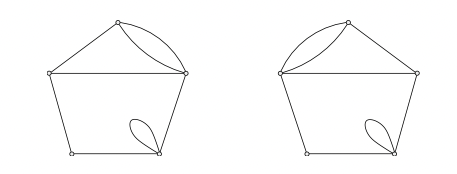
\includegraphics[scale=0.65]{pics/p1.2.2.png}
    \caption{Gráficas del \textbf{Problema 1.2.2}}
    \label{fig:p1.2.2}
\end{figure}

%---------------------------------------
\begin{problem}{1.2.2}

\end{problem}
\textit{Solución.} \textbf{Está fácil; solo hay que fijarnos en el vértice con un lazo.}
%---------------------------------------

%---------------------------------------
\begin{problem}{1.2.3}

\end{problem}
\textit{Solución.} Sea $G$ una gráfica conexa y sea $H$ una gráfica isomorfa a $G.$ Sean $X, Y \subset V(H)$ una partición del conjunto $V(H).$ Sea $\phi: G \rightarrow H$ el isomorfismo entre las gráficas $G$ y $H.$ Entonces, $\phi^{-1}(X)$, $\phi^{-1}(Y)$ es una partición del conjunto $V(G)$. Puesto que $G$ es conexa, existe una arista $e = xy$ en $G$ tal que $x \in \phi^{-1}(X)$ y $y \in \phi^{-1}(Y).$ Como $\phi$ es un isomorfismo, $\phi(e) = \phi(x) \phi(y)$ es una arista en $H$ con un extremo en $X$ y otro en $Y.$ Como la partición $X,Y$ de $V(H)$ fue arbitraria, lo anterior muestra que $H$ es conexa.
%---------------------------------------

\begin{figure}
    \centering
    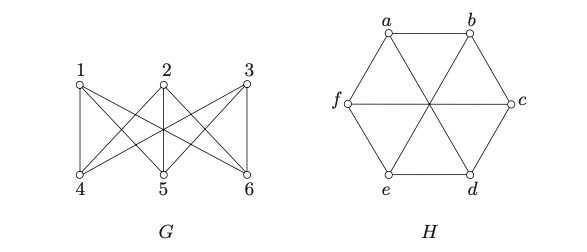
\includegraphics[scale=0.65]{pics/p1.2.4.png}
    \caption{Gráficas del \textbf{Problema 1.2.4}}
    \label{fig:p1.2.4}
\end{figure}

%---------------------------------------
\begin{problem}{1.2.4}

\end{problem}
\textit{Solución.} \begin{itemize}
    \item[a)]  \textbf{Tedioso}
\end{itemize}
%---------------------------------------

%---------------------------------------
\begin{problem}{1.2.6}

\end{problem}
\textit{Solución.} \textbf{Tedioso}
%---------------------------------------

%---------------------------------------
\begin{problem}{1.2.7}

\end{problem}
\textit{Solución.} Ver Tarea 1.
%---------------------------------------

%---------------------------------------
\begin{problem}{1.2.10}

\end{problem}
\textit{Solución.} \begin{itemize}
    \item[a)] Sea $P_n = v_1 \cdots v_n$ un camino en $n$ vértices. Sea $\phi: P_n \rightarrow P_n$ un automorfismo. Puesto que $\phi$ preserva los grados de los vértices, $\phi(v_1) = v_1$ o $\phi(v_1) = v_n.$ Considere primero el caso $\phi(v_1) = v_1.$ Puesto que $\phi$ preserva incidencias, se tiene que $\phi(v_1) \phi(v_2) = v_1 \phi(v_2) = v_2$. Inductivamente, suponga que $\phi(v_j) = v_j$ para toda $j < n.$ Entonces, dado que $\phi$ es un automorfismo, $\phi(v_{n-1})\phi(v_n) = v_{n-1} \phi(v_n) = v_{n-1} v_n.$ Por tanto, en este caso, $\phi$ es el automorfismo identidad.
    
    Ahora suponga que $\phi(v_1) = v_n$. Dado que $\phi$ preserva inicidencias, $\phi(v_1) \phi(v_2) = v_n \phi(v_2) = v_n v_{n-1}$. Inductivamente, suponga que $\phi(v_j) = v_{n-j+1}$ para $j < n.$ Luego, puesto que $\phi$ es un automorfismo, $\phi(v_{n-1})\phi(v_n) = v_2 \phi(v_n) = v_2 v_1$. Por tanto, $\phi$ es el automorfismo determinado por la regla $v_j \mapsto v_{n-j +1.}$ Note que, en este caso, $\phi \circ \phi = id$.
    
    Por tanto, el grupo de automorfismos de $P_n$ consta de dos elementos, es decir, es isomorfo a $S_2.$
    \item[b)] \textbf{Falta mostrar muchas cosas}
\end{itemize}
%---------------------------------------

%---------------------------------------
\begin{problem}{1.2.11}

\end{problem}
\textit{Solución.} Sea $\phi: G \rightarrow G$ un automorfismo. Note que por definición, $V(G) = V(\overline{G}).$ Entonces $\phi$ es una biyección en los vértices de $\overline{G}.$ Si $xy$ no es una arista en $G$, entonces $\phi(x) \phi(y)$ no es una arista en $G.$ Pero esto implica que la arista $xy$ en $\overline{G}$ se mapea mediante $\phi$ a una arista $\phi(x) \phi(y)$ en $\overline{G.}$ Por tanto, $\phi$ es un automorfismo de $\overline{G}$. Por tanto todo automorfismo de $G$ es un automorfismo de $\overline{G}$. Más aún, por simetría, todo automorfismo de $\overline{G}$ es un automorfismo de $G.$ Se concluye que $Aut(G) = Aut(\overline{G}).$ \textbf{Falta mejorar redacción.}
%---------------------------------------

%---------------------------------------
\begin{problem}{1.2.13}

\end{problem}
\textit{Solución.} Ver tarea 1.
%---------------------------------------

%---------------------------------------
\begin{problem}{1.2.14}

\end{problem}
\textit{Solución.} \begin{itemize}
    \item[a)] Sea $G$ una gráfica simple. Si $n = 2$, entonces $G$ es $K_2$ o $G = K_1 \cup K_1$. En ambos casos, $Aut(G) = S_2$, por lo que $G$ no es asimétrica.
    
    Ahora bien, si $n = 3$, entonces tenemos que $G = K_1 \cup K_1 \cup K_1$ o  $G = K_2 \cup K_1$ o $G = P_3$ o $G = K_3.$
    \textbf{NO ME GUSTA ESTE ARGUMEMTO; MUCHA TALACHA}
    
    \item[b)]
\end{itemize}
%---------------------------------------

%---------------------------------------
\begin{problem}{1.2.17}

\end{problem}
\textit{Solución.} Ver tarea 1.
%---------------------------------------

%---------------------------------------
\begin{problem}{1.3.2}

\end{problem}
\textit{Solución.}
%---------------------------------------

%---------------------------------------
\begin{problem}{1.3.4}

\end{problem}
\textit{Solución.}
%---------------------------------------

%---------------------------------------
\begin{problem}{1.3.7}

\end{problem}
\textit{Solución.}
%---------------------------------------



%---------------------------------------
\begin{problem}{1.3.8}

\end{problem}
\textit{Solución.} Ver Tarea 1
%---------------------------------------


%---------------------------------------
\begin{problem}{1.4.1}

\end{problem}
\textit{Solución.}
%---------------------------------------


%---------------------------------------
\begin{problem}{1.4.5}

\end{problem}
\textit{Solución.}
%---------------------------------------


%---------------------------------------
\begin{problem}{1.4.6}

\end{problem}
\textit{Solución.}
%---------------------------------------

\section*{Capítulo 2}


%---------------------------------------
\begin{problem}{2.1.1}

\end{problem}
\textit{Solución.} Sea $\mathcal F$ la familia de subgráficas conexas maximales de $G.$ Sea $H$ una componente conexa de $G.$ Note que 
%---------------------------------------



%---------------------------------------
\begin{problem}{2.1.2}

\end{problem}
\textit{Solución.} \begin{itemize}
    \item[a)] Si $n = 2$, entonces $G$ es isomorfa a $P_2$ o a $K_1 \cup K_1$. En ambos casos, $G$ tiene dos vértices de grado menor que dos. Suponga, inductivamente, que toda gráfica acíclica que no es trivial con menos de $k$ vértices tiene dos vértices de grado menor que dos. Sea $G$ una gráfica con $k$ y acíclica. Como es acíclica, existe un vértice $u$ de grado uno.  Haga $H = G \setminus u$, y note que $H$ también es acíclica, pues es subgráfica de $G.$ Como $H$ tiene $k-1$ vértices, la hipótesis de inducción establece que existen dos vértices $v_1, v_2$ en $H$ con grado menor que dos en $H.$ Note que a lo más uno de estos, digamos $v_1$, es vecino de $u$ en $G,$ pues esté vértice es de grado uno en $G.$ Por tanto, $v_2$ también es de grado menor que dos en $G$ y junto con $u$ se tienen dos vértices de grado menor que dos. 
    \textbf{Mejorar redacción.}
    \item Sea $G$ es conexa, acíclica y no trivial. El inciso a) establece que existen dos vértices $u, v$ en $G$ de grado menor que dos. La conexidad de $G$ implica que todos sus vértices tienen grados positivos. Así, pues, los vértices $u,v$ tienen grado uno en $G.$
    
   % Si $G$ tiene únicamente dos vértices de grado uno, entonces $G$ es isomorfa a $P_n$. Para ver esto, sea $P$ el camino más largo contenido en $G.$ Como $G$ es acíclica, los vértices iniciales y finales en $P$ son de grado uno en $G$ (los únicos). Haga $X =  G \setminus P$ y supnga que $X \neq \varnothing$. Como $G$ es conexa, existe arista $e = xy$ con $x \in X$ y $y \in P.$
   \textbf{FALTA}
    \end{itemize}
%---------------------------------------


%\printbibliography

\end{document}